\documentclass[a4paper,12pt]{article}
\pagestyle{plain}

\usepackage{graphics}
\usepackage{graphicx}
\usepackage{grffile}
\usepackage{epsfig}
\usepackage{rotating}
\usepackage{euscript}
\usepackage{eufrak}
\usepackage{color}
\usepackage{amsmath}
%\usepackage{amssymb}
\usepackage{multirow}  


\parindent      = 0.0in
\parskip        = 0.08in
\widowpenalty   = 10000
\clubpenalty    = 10000
\labelsep       = 0.1cm
\itemsep        = 0.0cm

\textheight 24cm
\textwidth  15cm
\oddsidemargin 0.in
\evensidemargin 0.in
\topmargin -0.25in
\footskip 0.75in
\headheight 0.in
\renewcommand{\bottomfraction}{1.0}
\renewcommand{\topfraction}{1.0}
\renewcommand{\textfraction}{0.0}

\def\st{\scriptstyle}
\def\sst{\scriptscriptstyle}
\def\mco{\multicolumn}
\def\epp{\epsilon^{\prime}}
\def\vep{\varepsilon}
\def\ra{\rightarrow}
\def\vp{{\bf p}}
\def\al{\alpha}
\def\ab{\bar{\alpha}}
\def\be{\begin{equation}}
\def\ee{\end{equation}}
\def\bea{\begin{eqnarray}}
\def\eea{\end{eqnarray}}

% Title Page
\title{First Year Report}
\author{Stefanie Lewis 0706250}


\begin{document}
\maketitle

\begin{abstract}

\end{abstract}

\newpage
\tableofcontents

\newpage

\section{Introduction}
This PhD project is focused on the development of analysis techniques to be used in the extraction of polarisation observables in the N* program at CLAS.  
%%%%EDIT THIS
Within the last 7 months, much time has been spent on getting accustomed to various aspects of the physics research environment.  Several new topics were explored; primarily Bayesian analysis (specifically Nested Sampling), object-oriented programming and baryon spectroscopy.  
\newline
A toy nested sampling program in C was provided and explored in order to become familiar with the algorithm.  The source code was then used to create a similar object-oriented program.  This provided an opportunity to not only introduce the concept of object orientation (specifically C++), but also to check the functional capabilities against those of the original C program.  Once the object-oriented program provided acceptable results, it was generalised in order to be applied to a variety of problems.  
\newline
The generalised program was then used to extract simplified spin observables from simulated data. This provided the opportunity to fine-tune the program and find any problems with the program. At this point, it was discovered that the program had an exceedingly long run-time when a high number of iterations were used, despite optimisation efforts.  The possibility of applying some of the programming techniques used in graphics processing units (GPUs) will be considered as a potential solution to the long run-time.
\newline
%Insert wee paragraph on shifts at JLab and various training exercises.
In addition to becoming accustomed to the computational skills, there has been some introduction to Jefferson Lab and the CLAS Collaboration.  A collaboration meeting in Paris was attended and a probationary membership to the collaboration has been approved.  Several training courses and exercises were done in preparation for shiftwork at Jefferson Lab's Experimental Hall B, including General Safety, Radiation Worker Safety and Oxygen Deficiency Hazard training.  



\section{Background}
\subsection{Baryon Spectroscopy and Spin Observables} 
%Baryon paper - Klempt, Richard
Despite the physics taught in undergraduate physics courses, the quark contributions to the spin of a nucleon are not well understood.  There exist several quark models which each attempt to provide an explanation of the spin nature of nucleons.  Baryon spectroscopy is an experimental approach used to support or preclude predicted quark models.  

%%%%This is from the Spin Observables section (which used to exist).  ABOVE HERE need to explain physics.
In order to become accustomed with the correlations and behaviour of spin observables, a small standalone program was created.  The aim of this macro was to generate dummy variables used to calculate the sixteen spin observables and output plots showing correlations between various observables.
\newline
Eight values were randomly generated from a Gaussian distribution over the surface of an 8-sphere.  These values were then combined to create four normalised complex amplitudes, $a_{1}$ to $a_{4}$.  Dummy values for these sixteen observables were calculated based on the expressions given in Table 1 below:
\newline
  \begin{center}
  \begin{table}[!h]
  \caption{Spin Observables in terms of Complex Amplitudes\cite{info}}
  \centering
  \begin{tabular}{c  c  c}
  \hline \hline
  Observable & Type & Amplitude Combination \\ [0.5ex]
  \hline \\
  $B$ & Single & $|a_{1}|^{2} + |a_{2}|^{2} - |a_{3}|^{2} - |a_{4}|^{2}$ \\
  $R$ & & $|a_{1}|^{2} - |a_{2}|^{2} + |a_{3}|^{2} - |a_{4}|^{2}$ \\
  $T$ & & $|a_{1}|^{2} - |a_{2}|^{2} - |a_{3}|^{2} + |a_{4}|^{2}$ \\ \\
  $E$ & Beam-target & $2\Re(a_{1}a_{3}^{*} + a_{2}a_{4}^{*})$ \\
  $F$ & & $2\Im(a_{1}a_{3}^{*} - a_{2}a_{4}^{*})$ \\ 
  $G$ & & $2\Im(a_{1}a_{3}^{*} + a_{2}a_{4}^{*})$ \\ 
  $H$ & & $-2\Re(a_{1}a_{3}^{*} - a_{2}a_{4}^{*})$ \\ \\
  $C_{x}$ & Beam-recoil & $-2\Im(a_{1}a_{4}^{*} - a_{2}a_{3}^{*})$ \\
  $C_{z}$ & & $2\Re(a_{1}a_{4}^{*} + a_{2}a_{3}^{*})$ \\
  $O_{x}$ & & $2\Re(a_{1}a_{4}^{*} - a_{2}a_{3}^{*})$ \\
  $O_{z}$ & & $2\Im(a_{1}a_{4}^{*} + a_{2}a_{3}^{*})$ \\ \\
  $T_{x}$ & Target-recoil & $2\Re(a_{1}a_{2}^{*} - a_{3}a_{4}^{*})$ \\
  $T_{z}$ & & $2\Im(a_{1}a_{2}^{*} - a_{3}a_{4}^{*})$ \\
  $L_{x}$ & & $-2\Im(a_{1}a_{2}^{*} + a_{3}a_{4}^{*})$ \\
  $L_{z}$ & & $2\Re(a_{1}a_{2}^{*} + a_{3}a_{4}^{*})$ \\ [1ex]
  \hline
  \end{tabular}

  \end{table}
  \end{center}
  %Insert table from Ireland's 

Histograms were generated such that each observable was plotted against each other observable in order to determine any correlations between them.  

\begin{figure}[!h]
 \begin{center}
  \includegraphics[scale=0.5]{histograms2D.eps}
  \caption{Observables were plotted against each other to show relationships between sets of observables.}
 \end{center}
\end{figure}

Plots showing circular patterns indicated that the two observables present in the histogram had a spherical correlation.  These have been documented in papers such as \cite{info}. A significant number of plots showed rectangular patterns.  Pairs of observables that formed such a pattern were listed in order to find sets of three observables in which every possible pair constituted a rectangularly distributed histogram.  Thirteen such triples were found, and when plotted in three dimensions, formed a tetrahedron.

\begin{figure}[!h]
 \begin{center}
  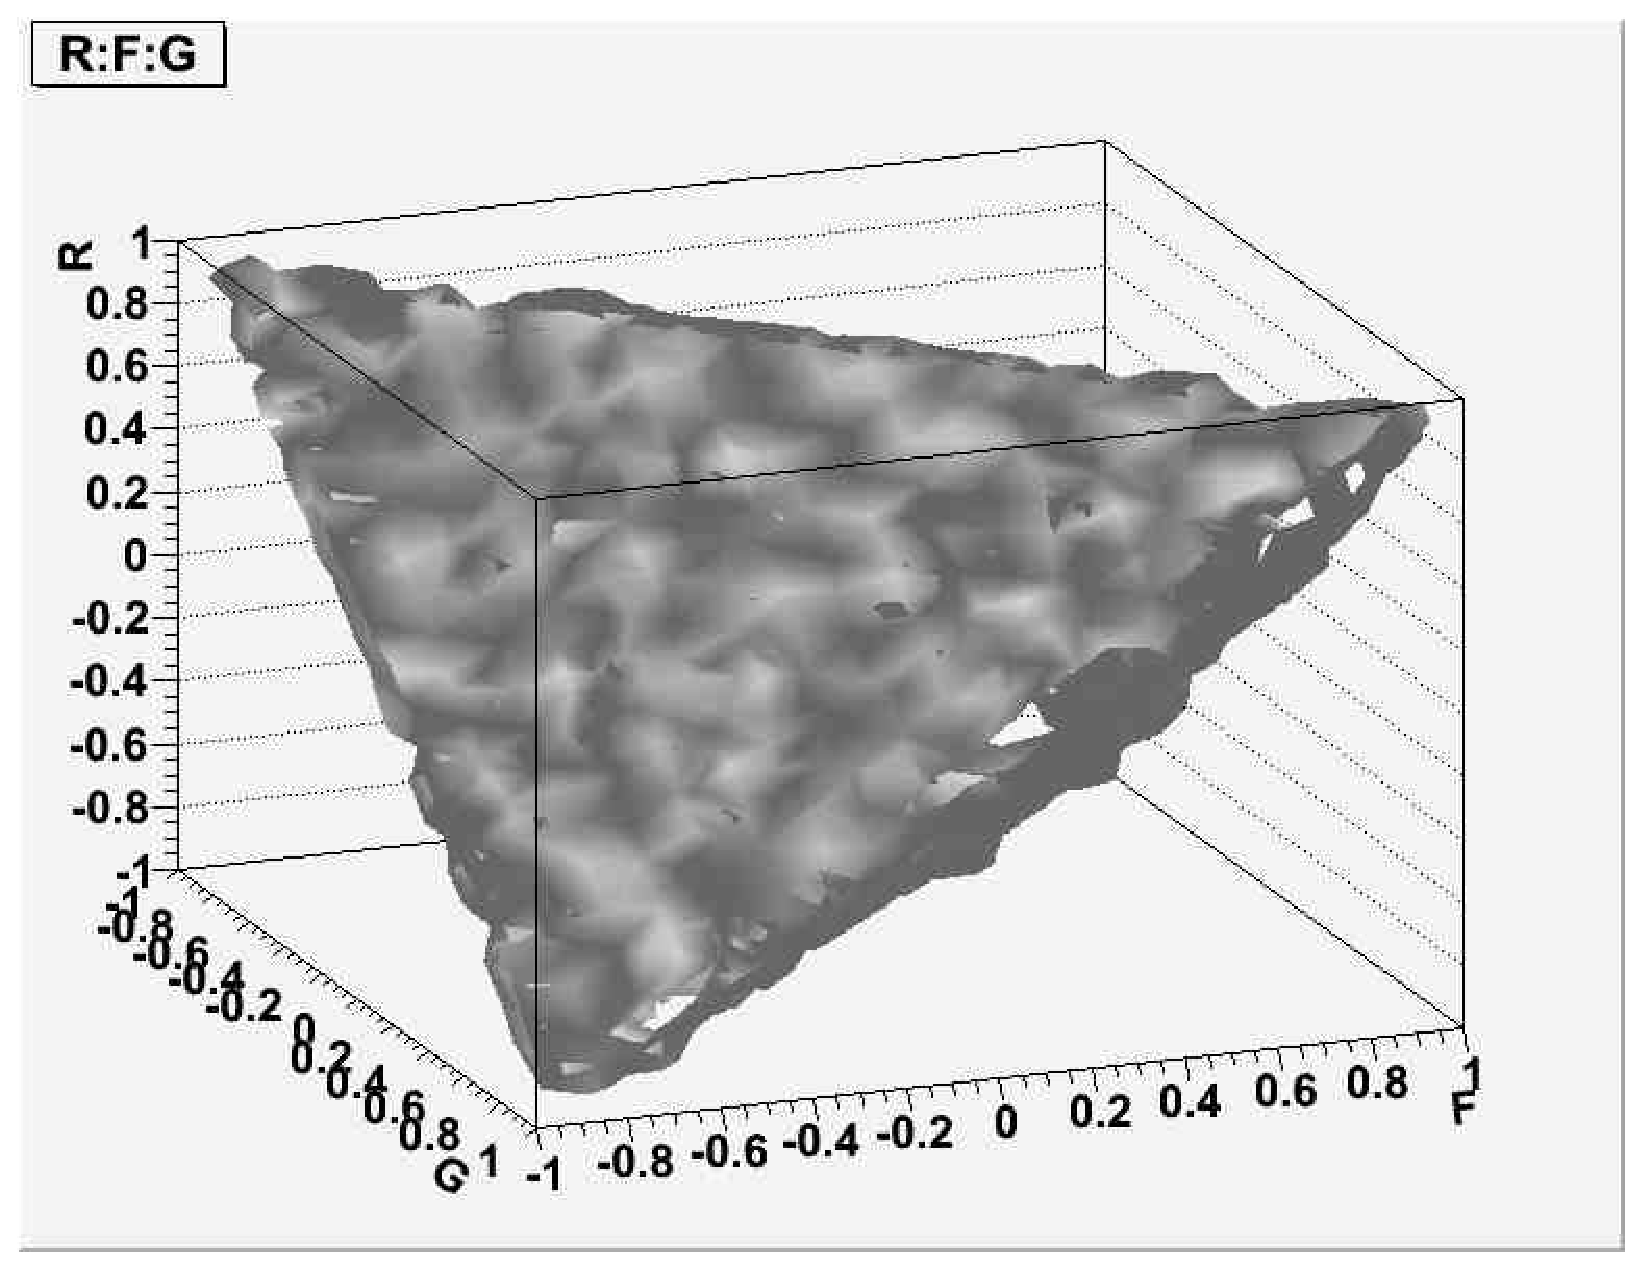
\includegraphics[scale=0.3]{RFG.eps}
  \caption{Tetrahedron resulting from plotting R, F and G in three dimensions.}
 \end{center}
\end{figure}

The equations defining the thirteen tetrahedra are shown below.


\begin{figure}[!h]
 \begin{center}
  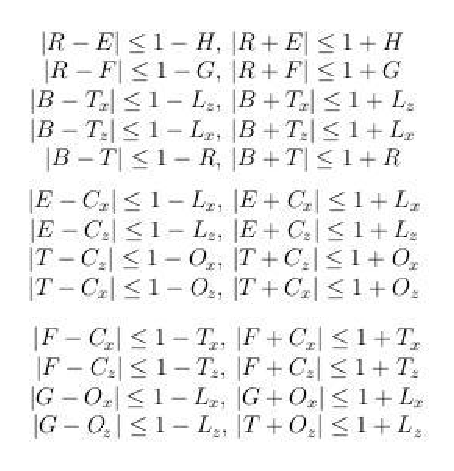
\includegraphics[scale=0.75]{ineqs.eps}
  \caption{The thirteen tetrahedral correlations correspond to the following triples: $REH, RFG, BT_{x}L_{z}, BT_{z}L_{x}, BTR, EC_{x}L_{x}, EC_{z}L_{z}, TC_{z}O_{x}, TC_{x}O_{z}, FC_{x}T_{x}, FC_{z}T_{z}, GO_{x}L_{x}$ and $GO_{z}L_{z}$.}
 \end{center}
\end{figure}

The significance of these thirteen triples is still being explored.

\subsection{CLAS at Jefferson Lab}
The CEBAF Large Acceptance Spectrometer (CLAS) Collaboration is based in Hall B of Jefferson Lab.  

\subsection{Nested Sampling}
%Sivia, Skilling
Nested sampling is a modern model comparison technique based on the principles of Bayesian statistics.  Most conventional analysis tools rely on the more widely known frequentist approach. In this approach, data is collected, and values such as the mean and standard deviation are extracted.  Any inferences are then based on the distribution of these statistics.  As such, the results are only based on a probability, and are not themselves probability statements.  The frequentist approach does not involve any knowledge or expectation of the results, and this is the key difference between frequentist and Bayesian statistics. \cite{bayes}
\newline
Bayesian statistics involves making an estimation of the results prior to any calculations.  This 'guess' is used to form a distribution with a easily determined mean and variance, known as the 'Prior'.  Bayes' Theorem (Eqn 1) is then used to combine the prior distribution with the data and produce a posterior distribution, the statistics of which determine the resulting mean, variance, etc. \cite{sivia} 
\newline

\begin{equation}
 prob(X|Y,I) = \frac{prob(Y|X,I) \times prob(X|I)}{prob(Y|I)}
\end{equation}
where I denotes any background information, X and Y are propositions, and $prob(X|Y,I)$ denotes the probability of X given Y and I.

The idea of Bayesian statistics can be expressed in the form of a simple equation \cite{skilling}:

\begin{equation}
 Prior \times Likelihood \longrightarrow Evidence \times Posterior
\end{equation}
where
\begin{equation}
 Prior = \pi(\theta)d\theta 
\end{equation}
\begin{equation}
 Likelihood = L(\theta)
\end{equation}
\begin{equation}
 Evidence = Z = \int LdX
\end{equation}
\begin{equation}
 Posterior = p(\theta)d\theta
\end{equation}

and
\begin{equation}
 dX = \pi(\theta)d\theta
\end{equation}

The prior is a distribution, or set of points that act as an initial starting point, an estimation or expectation of the results.  Each point has an associated likelihood determined by a likelihood function.  This is usually dependent on the applicable data.  If, for example, in an effort to determine the x-coordinate of an object, the prior would consist of a set of possible x-coordinates.  The likelihood associated with each point describes how likely that point is the x-coordinate of the object.
\newline
The output of a Bayesian calculation contains two pieces. The evidence, $Z$, is useful in comparing model assumptions.  Bayes factors, or ratios of evidence, are used to compare any two models at any time without the need to recalculate anything \cite{skilling}. The posterior is the distribution of points that result from the calculation.  These posterior points are determined primarily by the prior and likelihood.
\newline
Nested sampling is unique in that it extracts both parts of the Bayesian output.  For a specific problem, a prior is determined, as well as a problem-specific likelihood function.  Each point in the prior is assigned a likelihood value based on the likelihood function.  The nested sampling algorithm then finds the point with the lowest likelihood, i.e. the 'worst' point. A weight is determined for this worst point. Two values are then calculated - the natural log of the evidence, $log(Z)$, and the \textit{information} $H$, defined below \cite{sivia}.
\begin{equation}
 H = \int log(\frac{dP}{dX})dP
\end{equation}
where $dP$ is the posterior.  The values associated with the point - the point itself, its likelihood and its weight are all stored in the posterior.  The worst object is then overwritten with a copy of a 'surviving' point (any point other than the worst).  This copy is then slightly altered, usually by adding a small randomly generated number.  The likelihood of this 'new' point is then calculated and compared to that of the 'worst' object.  If it is found to be lower than the previously determined lowest likelihood, the new point is altered again.  This process uses an MCMC to ensure that the resulting new point is only a slight change from a surviving point, and that its likelihood is at least higher than that of the overwritten 'worst' object.
\newline
This process is iterated through for either a predetermined number of iterates or until some termination condition is met.\cite{skilling,sivia}
\newline
The following diagram shows the process of nested sampling pictorially.  In this example, an object is placed at x = 3.  The prior consists of a set of x values distributed linearly on the interval (0,5).  The likelihood of the object being found at a given x-position is defined by the function below.
\begin{equation}
 L = 6x - x^{2} - 2
\end{equation}
The distribution of the points after each iterate of the nested sampling algorithm is shown in each line of the diagram below.


\begin{figure}[!h]
 \begin{center}
  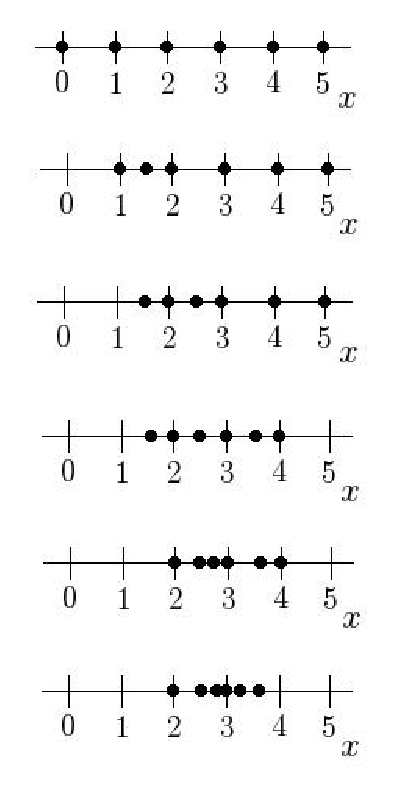
\includegraphics[scale=0.75]{nsdiagram.eps}
  \caption{After each iterate, the values begin converging on 3 - the position of the object.}
 \end{center}
\end{figure}

%Start by briefly describing the basic difference between the frequentist approach and Bayesian probability.
%Show equations used, in particular, Bayes' Theorem.
%Important to clearly explain all terms such as Prior, Posterior, Evidence, etc.

%This section could just follow on naturally from the last section, include equations and any diagrams that may help.


\section{Nested Sampling}
\subsection{The Lighthouse Problem}
In order to become accustomed with both programming and the concept of Nested Sampling, a toy problem from \cite{sivia} was attempted: \\ \\
\textit{``A lighthouse is somewhere off a piece of straight coastline at a position $\alpha$ along the shore and a distance $\beta$ out at sea. It emits a series of short highly collimated flashes at random intervals and hence at random azimuths. These pulses are intercepted on the coast by photo-detectors that record only the fact that a flash has occurred, but not the angle from which it came. \textbf{N} flashes have so far been recorded at positions $x_{k}$. Where is the lighthouse?''}\cite{sivia}
\\ \\



\begin{figure}[!h]
 \begin{center}
  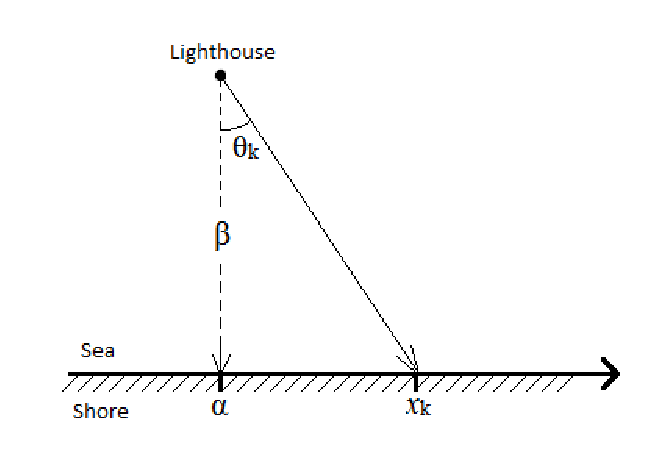
\includegraphics[scale=0.75]{lighthouse.eps}
  \caption{Diagram of Sivia's Lighthouse Problem \cite{sivia}}
 \end{center}
\end{figure}


The 64 values of $x_{k}$ were previously generated with the lighthouse being positioned at (1,1) and were provided by \cite{sivia}.

Source code in C was provided and used to create an object-oriented program in C++.  The results of both approaches were compared and found to be equivalent, which ensured the functionality of the C++ version of the program.  The purpose of using object orientation was to ensure that the program was as generic as possible in order for it to be applied to other problems.  Several methods, however, were problem-specific.
\newline
     
The prior was assumed to be uniform on x = (-2,2) and y = (0,2).  That is, arrays of x and y coordinates were filled with values randomly generated on (0,1) and mapped to the intervals (-2,2) and (0,2) respectively.  Each (x,y) point was then used to calculate a likelihood value that reflected the probability of the lighthouse being situated at those coordinates.
\newline

\begin{equation}
 LogL = \sum log(\frac{(y/\pi)}{(D[k]-x)^{2} + y^{2}})
\end{equation}
where D is the array of flash positions $x_{k}$ and the expression is summed from k = 0 to 63.


%\newline 
The nested sampling algorithm is then run using the calculated likelihood values.  During each iteration, the Explore() function was called in order to overwrite the point with the lowest likelihood with an evolved copy of another point, as discussed in Section 2.2.  In this problem, small random numbers were added to the x and y values and a new likelihood was calculated.  If this new likelihood was less than that of the 'worst' object, it was rejected and the loop was run through again, with slightly larger random numbers added.  This loop, a Markov Chain Monte Carlo algorithm, was iterated twenty times in order to obtain a slightly altered copy of a surviving point with a likelihood greater than that of the overwritten point. 
\newline
The size of the prior (i.e. the number of samples used initially) and the number of iterates were altered in order to obtain an idea of the optimal set-up of the program.  The results of these tests are shown below.

%%%%%Insert no samples v no iterates

\begin{figure}[!h]
 \begin{center}
  \includegraphics[scale=0.5]{convergence.eps}
  \caption{Graph denoting the relation between number of objects (points) and number of iterates.  For each number of objects, the number of iterates at which the log of the evidence and the information were found not to change (i.e. the number of iterates required for them to converge) were plotted, respectively.}
 \end{center}
\end{figure}



Once a sufficient set of initial values was found, the results of the object-oriented program were compared to those obtained from the original C program.  The following plots show the comparison.  

%%%%%Insert results of both my code and Sivia's here.  Mention initial values in caption.  Also mention the position of the lighthouse (probably goes in a previous paragraph - where the data is mentioned).


\begin{figure}[!h]
 \begin{center}
  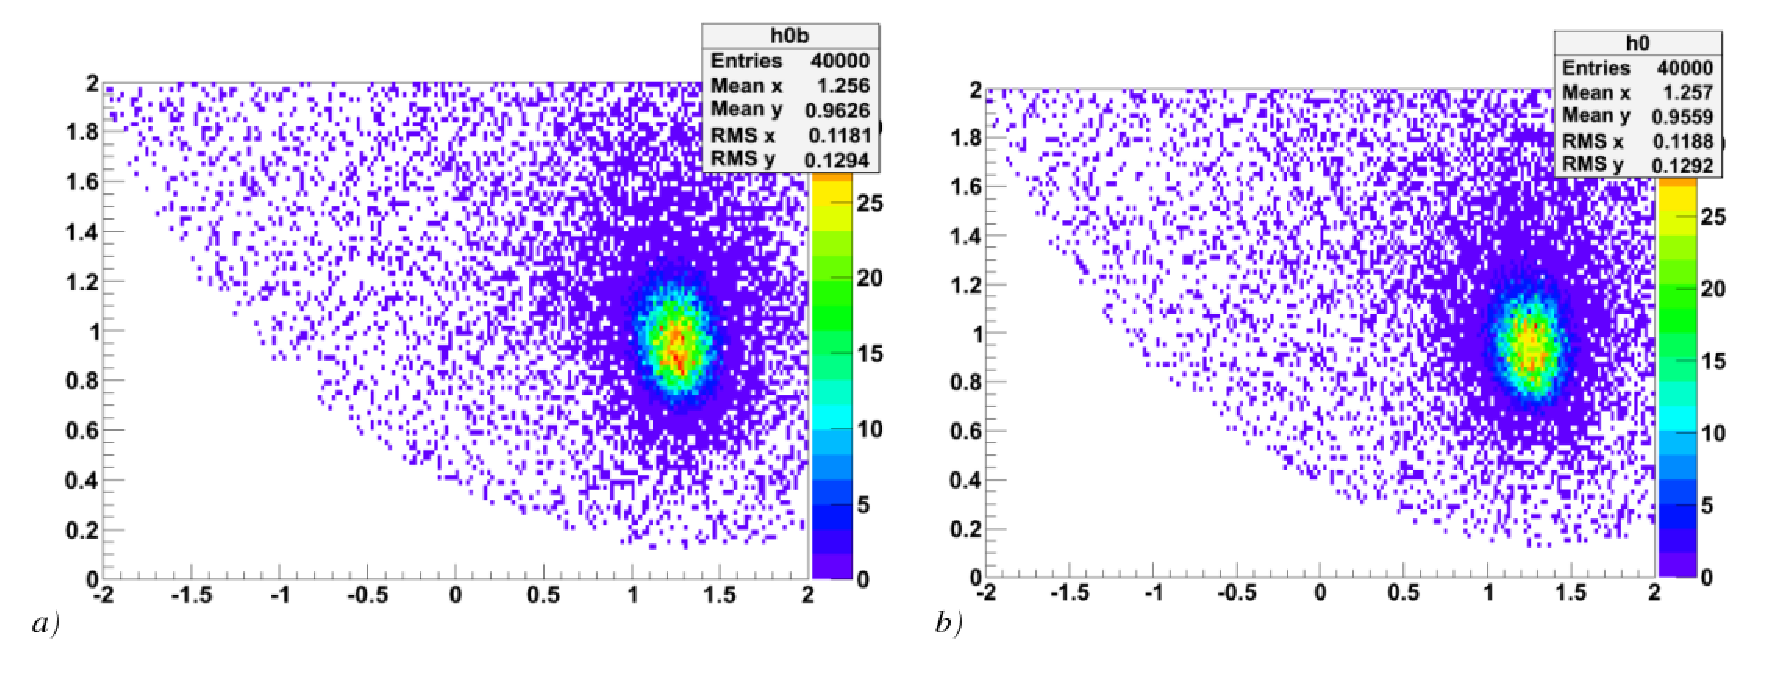
\includegraphics[scale=0.4]{lighthouseresults.eps}
  \caption{The results of running both versions of the code with the same initial values are shown above.  a) The C code provided by Sivia; b) The object-oriented C++ code.}
 \end{center}
\end{figure}

It was apparent from these plots that the two versions of the code were consistent with each other.  This test was used to ensure that the object-oriented version was functional to at least the same degree as the C code provided.  This was particularly useful in becoming familiar with programming in an object-oriented language.


 
\subsection{Applications to Baryon Spectroscopy}
%Describe prior, likelihood and explore functions used in program.

%%%%Need to cite CLAS note.
Once a working version of the generic object-oriented nested sampling program was achieved, it was applied to a more physics-related problem.  The first task in this physics application was to extract the value of one observable - the photon-beam asymmetry, B (defined in Table I). An event generator was used to generate dummy data, given a specific value for B.  This data consisted of azimuthal angles and polarisation states.
%%%%Polarisation of what???
\newline
In this case, each point in the prior was described by eight normalised values randomly generated from a Gaussian distributed over the surface of an 8-sphere, in a similar manner as described in Section 3. %Spin observable section.
These values were then combined to form four complex transversity amplitudes, which were used to calculate a value of B based on the expression in Table I.  The likelihood associated with each calculated value of B was determined by the equations below.
\begin{equation}
 \tilde{A} = \frac{P_{\gamma}B\cos2\phi + \delta L}{1 + P_{\gamma}B\cos2\phi \delta L}
\end{equation}


\begin{equation}
X = \frac{1}{2}(1 \pm \tilde{A})
\end{equation}

\begin{equation}
logL = \sum log(X)
\end{equation}
where $P_{\gamma}$ is the photon polarisation number, $\delta L$ is the luminosity asymmetry and $logL$ is the natural logarithm of the likelihood.  In Eqn. 6, %Middle one!
$\tilde{A}$ was added or subtracted based on whether the associated polarisation perpendicular or parallel, respectively.  These values were summed for all events - that is, all angles and polarisation states.  
\newline
These values were then used as usual in the nested sampling algorithm.  The Explore() function added a small randomly generated number to each of the eight initial values.  The small randomly generated number was determined by a Gaussian distribution of a set width.  This width was altered after each iteration of the MCMC loop in the function.  As per the Lighthouse example described in Section \textbf{Lighthouse}, a new likelihood value was calculated and compared to that of the 'worst' point in order to ensure that the new point was at least more likely than that which had been overwritten.  The results of the program were compared to the value of B input into the event generator.

%%%%%Insert results plots here.  Mention in caption number of iterates and samples.

\subsubsection{Evolved Prior}
%Describe evolved prior.  Need plots showing how prior and results evolve each time.
%Describe algorithm, show equations.
It was possible to add some complexity to the simple observable extraction program by using a previously generated posterior to confine the prior.  The posterior generated by the program contained tens of thousands of points (determined by the number of iterations) with unequal weights.  It was found that these points contained in the posterior could be used to generate a more accurate prior, rather than using random numbers from a Gaussian distribution on the surface on an 8-sphere.  A ``cumulant staircase'' was used to create an equally-weighted posterior\cite{sivia}.
%Insert diagram of cumulant staircase here.

%Describe method and equation.

\section{Analysis Program}
\subsection{SCons}
In the CLAS Collaboration at Jefferson Lab, a software construction tool called SCons\cite{scons} has become increasingly popular.  It is a simple, relatively easy-to-use alternative to the more commonly used Makefile.  The nested sampling program developed in this project was compiled using this SCons program.  SCons is scripted using Python, and is thus fairly intuitive to code.  The main file, required to be named 'sconstruct', imported any required Python scripts, listed the source code files to be compiled and any compiler flags required. Several Python scripts were imported in order to compile using ROOT libraries.  This provided a straightforward alternative to the complicated standard, autoconf.


 
\subsection{Structure and Coding}
An object-oriented (specifically C++) approach to the program was taken in order to make the nested sampling algorithm as generic as possible.  The program was comprised of two main classes, with a third acting as the user's front end (where various changes can be made). A combination of C++ and ROOT libraries were used.  
\newline

\begin{figure}[!h]
 \begin{center}
  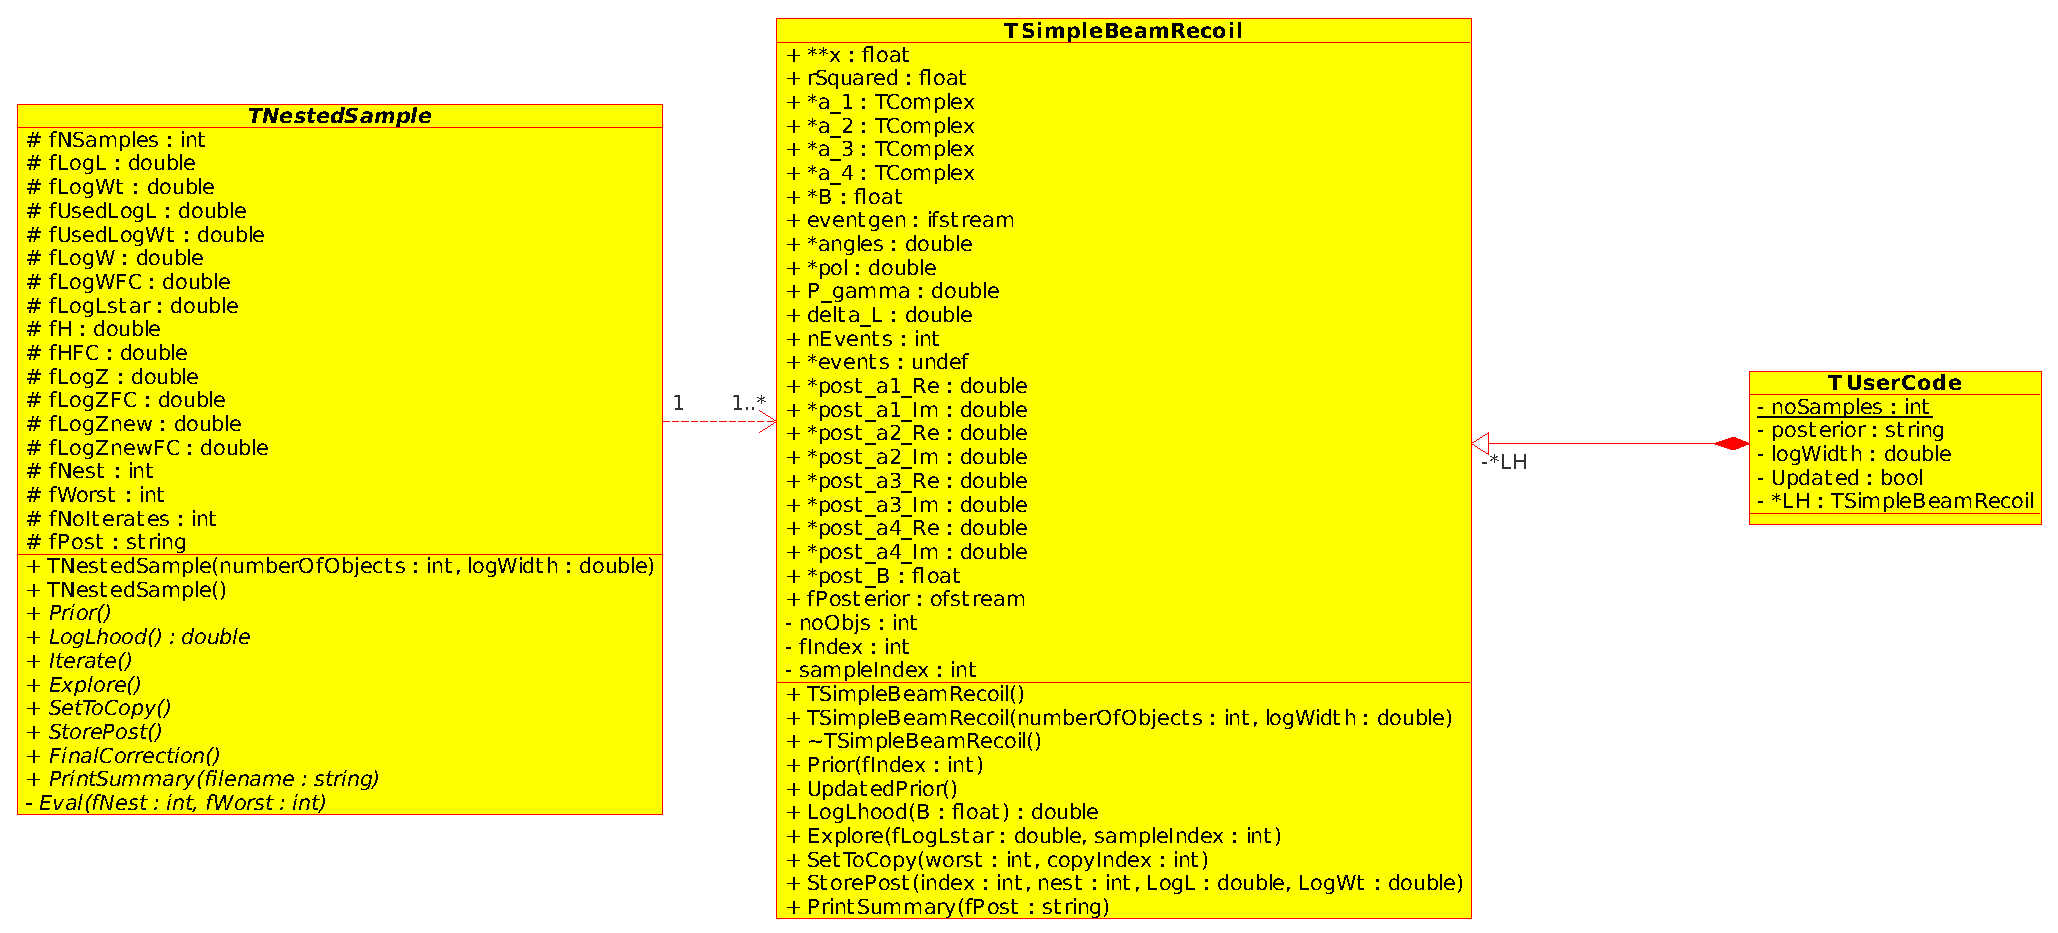
\includegraphics[scale=0.5]{class_diagram.eps}
  \caption{Class diagram showing methods, attributes and associations.}
 \end{center}
\end{figure}

An abstract class, TNestedSample, was used for defining the generic methods - Iterate(), Eval() and FinalCorrection().  These methods are responsible for the iteration over the nested sampling algorithm, termination and the nested sampling algorithm itself.  Other methods, such as Prior(), Explore() and PrintSummary(), must be defined for each derived class (i.e. for each application) as they are problem-specific.  The front end class, called TUserCode, determined which derived class would be used, called all required functions and set some initial values.  In principle, one could have multiple derived classes (i.e. applications to different problems) in one directory, and the user would be able to specify in TUserCode which derived class to use.  Each derived class would inherit the generic methods from the parent class.  For example, both Sivia's Lighthouse problem and the application to simple B observable extraction used the same abstract parent class - they differed solely in the derived classes.  
\newline
The nested sampling algorithm was contained in the Eval() method.  This private method was called from within the Iterate() method, which determined the number of iterations required in order to ensure a sufficiently precise result. A termination condition was determined based on work by Skilling\cite{skilling}.

%%%%%%%% Talk about termination condition here.

This termination condition ensured that the values for Log(Z) (the natural log of the evidence) and the information, H, differed only by a small amount respectively between iterations.  This could be written as ``The number of iterates should significantly exceed the product of the number of samples and the information H.''\cite{skilling}
\newline
In the program, this condition was implementing in a for loop as shown below:
\newline
\begin{verbatim}
 for (fNest = 0; fNest <= N*fNSamples*fH){
      // run code
  }
\end{verbatim}
where fNest is the number of iterations, fNSamples is the number of samples, fH is the information and N is an integer whose value can be changed.  

%\newline
An small, additional method was implemented called FinalCorrection().  This was intended to be an optional small correction to the calculations.  This method went through the samples, determined a log weight for each (much in the same way as in the core nested sampling algorithm - but did not require the program to find the point with the lowest log-likelihood) and calculated Log(Z) and H as normal.  The Explore() function was not called from this method as the samples were not changed.  The results were stored in the posterior as before.  

%%%%% I think this next piece should be in Performance Testing.
%\newline
This parameter, N, determined by how much the number of iterations exceeded the product of the number of samples and the information.  As N was increased, the accuracy of the program also increased, but so did the amount of time required for computation.  For this reason, it was important to determine a value of N that allowed for the program to be sufficiently accurate but also did not require an excessive amount of time to run.  In the case of the TSimplePhysics program described above, values of approximately 2-5 were found to be effective.


%%%%% Show termination condition plots here

\subsection{Output}
The nested sampling program generated an output in several forms.  Basic information about the running of the program was output to the screen, as shown in Figure 3.
%Insert wee screenshot of basic output to terminal.

\begin{figure}[!h]
 \begin{center}
  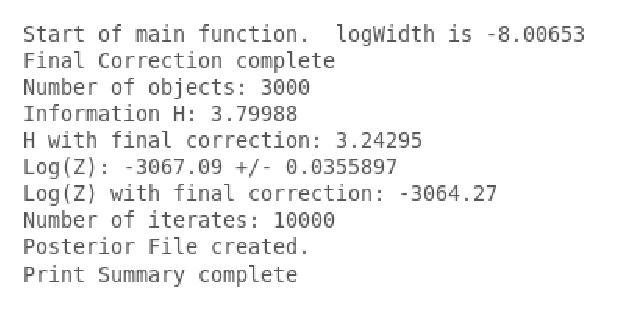
\includegraphics[scale=1]{term_output.eps}
  \caption{Information shown in terminal after running TSimplePhysics program.}
 \end{center}
\end{figure}

The standard deviation uncertainty for Log(Z) was printed (as shown in Fig. 4) based on the following equation provided by Sivia\cite{sivia}:
\begin{equation}
 \sigma = \sqrt{\frac{Information\  H}{Number\  of\  samples}}
\end{equation}


%Maybe briefly describe the terms that are output?
In addition to outputting to the screen, a ROOT tree (written to a .root file) was also created.  This tree was used to store many types of information in the form of branches.  The ROOT tree was used to examine the results visually.  A ROOT macro was written and used to generate several histograms showing the key results from the posterior.  Examples of these plots can be found in \textbf{SECTIONS WITH PLOTS}.


During testing of the program, additional text files were output in order to ensure that various sections of the code were working as intended.  In particular, the introduction of an evolved prior required several files to be created and examined in ROOT.


\subsection{Performance Testing}
Several performance tests were carried out on the program in order to determine its ability to extract the desired observables.  All tests were done using data simulated by an event generator.
\subsubsection{Event Generator}
%Describe event generator, briefly how it works.
\subsubsection{Timing Tests}
%Describe timing tests and implications.  GPU possibility here!!


\section{Conclusions}
\newpage

\section{Future Work}

Despite promising results, there is still much work to be done in the development of this Nested Sampling analysis program.  In the next twelve months, the program will be improved through a number of amendments.  Initially, the nested sampling program was simple and basic.  The level of complexity has been (and will continue to be) increased until it can be run on experimental data.  
The first step in this development is to handle all observables.  Instead of simply extracting the B observable, all sixteen observables will be extracted.  Calculations of statistical errors must also be included in the program.

Once this improvement has been implemented, it will be tested with data from experiment that has previously been studied.  The results will be compared to those obtained from a maximum-likelihood analysis program in order to ensure an acceptable level of accuracy. Once a sufficient degree of accuracy has been shown (and any necessary tweaks and adjustments have been made), the program will be used to evaluate new experimental data.

One of the drawbacks of this nested sampling approach is the excessive run-time required to obtain good results.  As discussed previously, this poses a significant problem.  The amount of time required to run the program using a sufficient number of iterations is longer than desired, despite optimisations.  The possibility of applying programming techniques used in graphics card programming and graphics processing unit (GPU) programming, in particular data parallelisation, will be strongly considered.  If successful, this would dramatically reduce the amount of time required to run the program with a high number of iterations. The implications of this improvement could enable the program to handle exceptionally large data sets in just minutes, making it a desirable alternative to maximum likelihood methods.

There will also be some involvement in the g14 (HDice) experiment at CLAS at Jefferson Lab. Any discrepancies in the tagger required to determine the photon energy will need to be found and calibrated.  This will involve using ROOTBEER, a program developed by Ken Livingston.  In order to perform this task, some time will also be spent becoming familiar with the software and various aspects of acquiring data files from the CLAS tape silos and farms. 


\begin{thebibliography}{99}
%biblio

\bibitem{skilling} J. Skilling, Bayesian Analysis 1 4, 833 (2006)
\bibitem{sivia} D. Sivia and J. Skilling, \textit{Data Analysis - A Bayesian Tutorial.} 2nd ed. Oxford Science Publications (2006)
%\bibitem{bayes} D. J. Bartholomew: A Comparison of Some Bayesian and Frequentist Inferences. Biometrika Issue 4 833-860, 2006
\bibitem{bayes} D. J. Bartholomew, Biometrika 52 (1-2), 19 (1965)
\bibitem{info} D. G. Ireland, Phys. Rev. C 82, 025204 (2010)
\bibitem{scons} The SCons Foundation, 2004. \textit{SCons: A Software Construction Tool.} [online] Available at: <http://www.scons.org> [Accessed 20 January 2011]
\end{thebibliography}

\end{document}          
